\chapter{Results}

Our proclaimed goals for the visualization was to enable large hierarchical networks in VR. 
Therefore, we tested our application in a performance evaluation in Section \ref{sec:performanceEvaluation} and gather different user feedback in the form of an informal evaluation (see Section \ref{sec:informalFeedback}) and heuristic evaluation (see Section \ref{sec:heuristicEvaluation}).

\section{Performance}
\label{sec:performanceEvaluation}

Real time 3D applications need to have a constant frame rate in order to achieve a smooth experience.
For VR-based applications this is even more important as a low frame rate could lead to motion sickness. 
In our performance test we distinguish between the average frame rate while the force based layout is being calculated when starting the application and the actual exploration phase. 
The exploration phase usually lasts for multiple minutes, while the initial layout calculation only lasts for a maximum of 1.5 minutes.
Therefore, we can assume a low performance during the layout calculation is not as critical as the exploration performance. 
The user can simply wait until the layout is completely finished.

In the performance evaluation we wanted to find out the quantity structure of the dataset. 
For an optimal VR experience the frame rate should be constant at the maximum of the supported Hz of the headset, for the HTC Vive this requires us to have 90 FPS.
Own experiences showed that 20-30 FPS is a minimum while exploring a virtual scene.
\\
We measured the FPS directly from the visualization by adding an FPS counter on the virtual controller model during the exploration. Our setup was a desktop PC with a Ryzen 7 3700X CPU and a Radeon RX 590 GPU. 
We tested multiple datasets with different sizes, the results are shown in Table \ref{table:resultFPS}. 
In order to detect possible performance problems we tested the scaling of the nodes and links individually as good as possible.
We found out that the number of nodes scale worse than the number of links (see Figure \ref{fig:performanceNodes} and \ref{fig:performanceLinks}). 
When we assume an equal distributed graph, the number of hierarchical layers only indirectly influence the frame rate, as with an increased number of layers the number of nodes grows exponentially. 
So before the application would run into performance problems based on the number of layers, the number of nodes would be too large anyway. 
In addition, with about 6 hierarchical layers the layout becomes unstable and can not guarantee a correct hierarchical nesting anymore.
\\
While the average frame rate is not drastically reduced by the links, the frame rate stability gets a bit worse. 
This was especially noticeable during the teleportation animation. 
Although we do not know for sure, we assume the automated scaling reduced the frame rate quite significantly. During the animation the scale of nearly all objects in the scenes is updated on every frame.
The maximum of 90 FPS is due to the maximum of 90Hz panel of the HTC Vive.
\\
Therefore, we conclude that at the current state of implementation the can support datasets up to 1500 nodes and 3000 links depending on the used system. 
During the exploration the CPU and GPU utilization was not at maximum. We assume that the application is CPU bound and further limited by the singled threaded Javascript implementation.

\begin{table}[!hbt]
    \resizebox{\textwidth}{!}{%
    \centering
    \begin{tabular}{ | c | c | c | c | c | c | }
        \hline
        \textbf{nodes} & \textbf{links} &\textbf{layers} &\textbf{layout - avg FPS} &\textbf{expl. - min FPS} &\textbf{expl. - avg FPS}\\
        \hline
        310  & 0    & 3 & 40 & 90 & 90\\ \hline
        730  & 0    & 3 & 30 & 70 & 75\\ \hline
        1100 & 0    & 3 & 20 & 55 & 60\\ \hline
        1560 & 0    & 4 & 20 & 40 & 55\\ \hline
        2343 & 0    & 5 & 10 & 30 & 35\\ \hline
        774  & 387  & 3 & 20 & 60 & 70\\ \hline
        774  & 1548 & 3 & 20 & 55 & 70\\ \hline
        774  & 3870 & 3 & 10 & 40 & 60\\ \hline
        1560 & 3120 & 4 & 5  & 25 & 45\\ \hline
        1020 & 2040 & 4 & 10 & 40 & 60\\ \hline
     \end{tabular}}
     \caption{Results from performance measurement evaluation (expl. ... exploration). Test setup: Ryzen 7 3700X + Radeon RX 590.}
     \label{table:resultFPS}
\end{table}

\begin{figure}[!hbt]
    \centering
    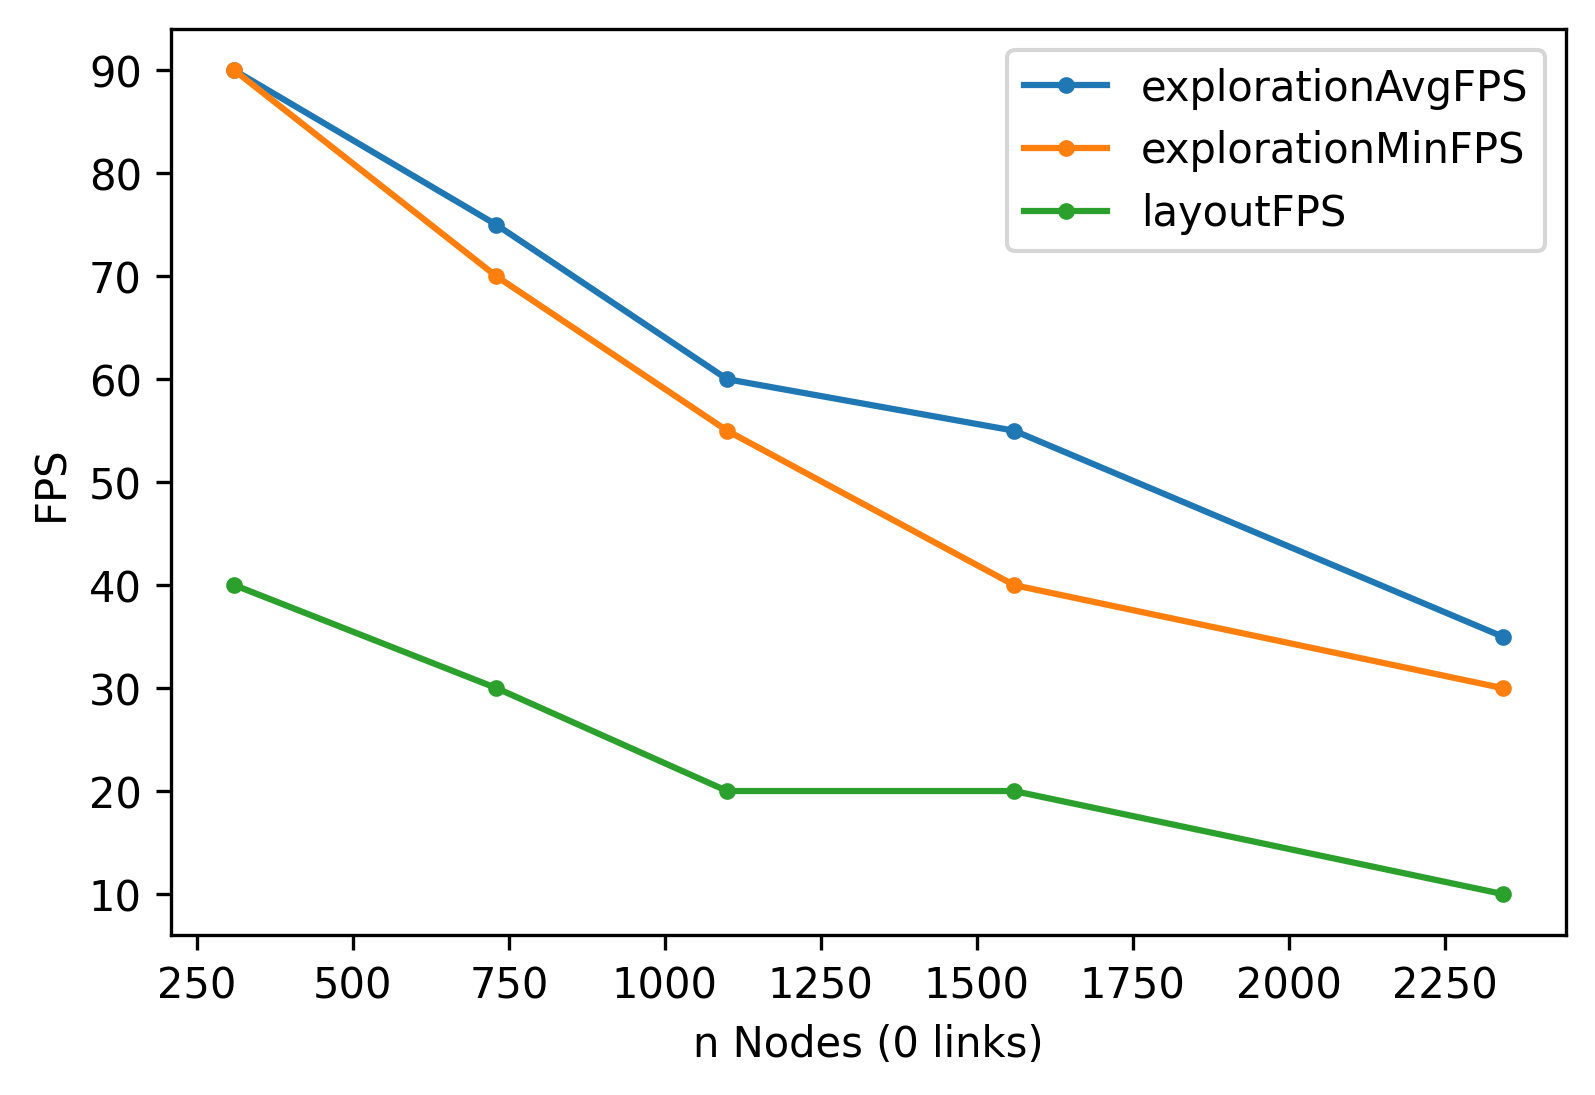
\includegraphics[width=0.75\textwidth]{graphics/performanceAnalysisNodes.png}
    \caption{Performance chart for scaling the number of nodes. To better compare the results only datasets with 0 links are shown in this graph. Increasing the number of nodes quickly leads to a performance issue.} 
    \label{fig:performanceNodes} 
\end{figure}

\begin{figure}[!hbt]
    \centering
    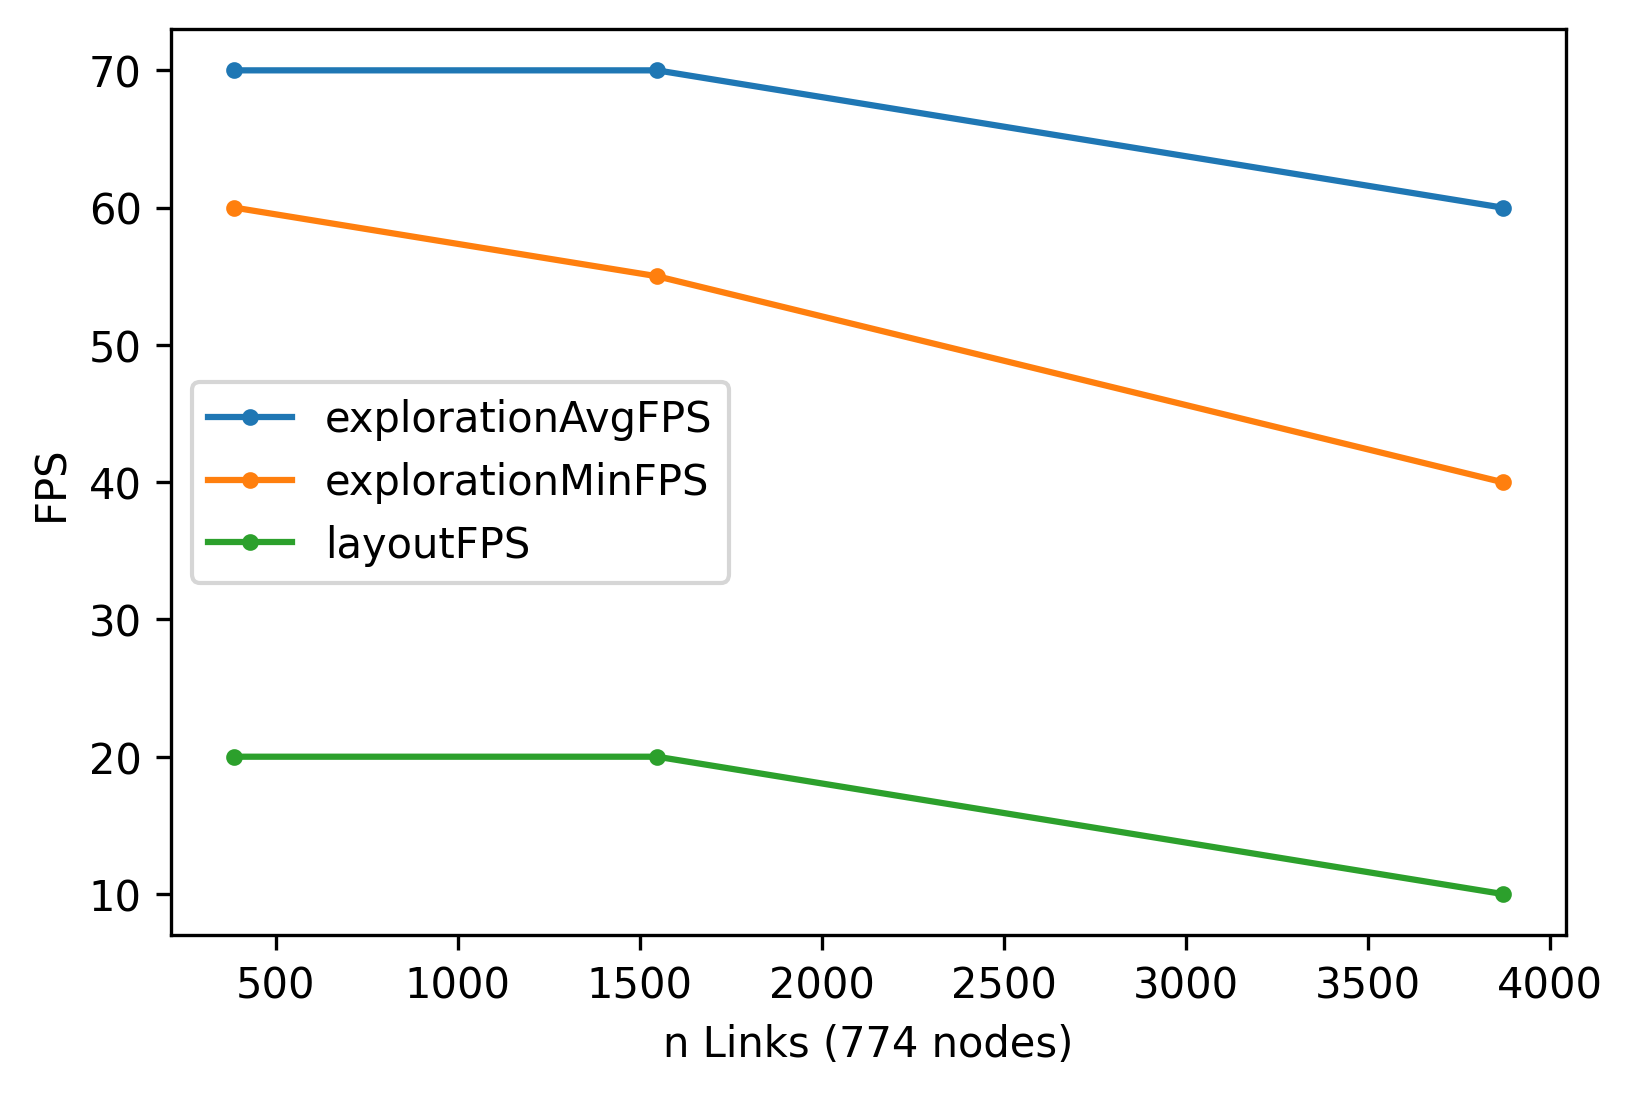
\includegraphics[width=0.75\textwidth]{graphics/performanceAnalysisLinks.png}
    \caption{Performance chart for scaling the number of links. To better compare the results only datasets with the same amount of 774 nodes are shown in this graph. In comparison to the nodes, links can be easier scaled up without impacting the performance too much.} 
    \label{fig:performanceLinks} 
\end{figure}

\subsection{Possible optimization}

To increase the overall performance the scalability for the number of nodes has to improve. We can separate the performance between GPU performance and CPU performance.
\\
For the GPU performance we already limit the draw calls by rendering the nodes with instanced buffers.
However, the number of rendered triangles is still very high. 
One improvement could be to use simpler spheres with a lower polygon count. Or implementing a technique that prevents the rendering of the small nodes which can not be seen anyway.
\\
To increase CPU performance we have to reduce the number of tasks during each iteration of the main render loop (see Figure \ref{fig:impl_programFlow}).
A big performance issues might be the ray casting. This could be improved by take advantage of the hierarchical layout. An intersection of child nodes from different parents than the one the user is currently inside is not possible anyways, therefore these nodes could be excluded from the ray intersection checks. 
Another improvement could be to bind the virtual laser pointer to a button that the user actively hold for its usage. 
That would enable an improved frame rate when the user is only looking around and not doing any interaction. 

\section{Informal feedback}
\label{sec:informalFeedback}

\subsection{Clarity of the visualization}
Filtering, visual clutter, hierarchical layout(intuitive?), ...

\subsection{Navigation}
Free fly, animated teleport, scaling, motion sickness.

\subsection{Interaction}
Button Mappings, Laser Pointer, 

\subsection{Performance}
Tested system and dataset

\section{Heuristic Evaluation}
\label{sec:heuristicEvaluation}